\documentclass[a4paper,10pt]{article}
\usepackage[utf8]{inputenc}
\usepackage{lipsum}

\usepackage[spanish]{babel}
\usepackage{fullpage}
\usepackage{cite}
\usepackage[utf8]{inputenc}
\usepackage{a4wide}
\usepackage{url}
\usepackage{graphicx}
\usepackage{caption}
\usepackage{float} % para que los gr\'aficos se queden en su lugar con [H]
\usepackage{subcaption}
\usepackage{wrapfig}
\usepackage{color}
\usepackage{amsmath} %para escribir funci\'on partida , matrices
\usepackage{amsthm} %para numerar definciones y teoremas
\usepackage[hidelinks]{hyperref} % para inlcuir links dentro del texto
\usepackage{tabu} 
\usepackage{comment}
\usepackage{amsfonts} % \mathbb{N} -> conjunto de los n\'umeros naturales  
\usepackage{enumerate}
\usepackage{listings}
\usepackage[colorinlistoftodos, textsize=small]{todonotes} % Para poner notas en el medio del texto!! No olvidar hacer. 
\usepackage{framed} % Para encuadrar texto. \begin{framed}
\usepackage{csquotes} % Para citar texto \begin{displayquote}
\usepackage{epigraph} % Epigrafe  \epigraph{texto}{\textit{autor}}
\usepackage{authblk}
\usepackage{titlesec}
\usepackage{varioref}
\usepackage{bm} % \bm{\alpha} bold greek symbol
\usepackage{pdfpages} % \includepdf
\usepackage[makeroom]{cancel} % \cancel{} \bcancel{} etc
\usepackage{wrapfig} % \begin{wrapfigure} Pone figura al lado del texto
\usepackage{mdframed}
\newcommand{\vm}[1]{\mathbf{#1}}
\newcommand{\N}{\mathcal{N}}

\newcommand{\citel}[1]{\cite{#1}\label{#1}}
\newcommand\hfrac[2]{\genfrac{}{}{0pt}{}{#1}{#2}} %\frac{}{} sin la linea del medio

 % imports varios
% tikzlibrary.code.tex
%
% Copyright 2010-2011 by Laura Dietz
% Copyright 2012 by Jaakko Luttinen
%
% This file may be distributed and/or modified
%
% 1. under the LaTeX Project Public License and/or
% 2. under the GNU General Public License.
%
% See the files LICENSE_LPPL and LICENSE_GPL for more details.

% Load other libraries

%\newcommand{\vast}{\bBigg@{2.5}}
% newcommand{\Vast}{\bBigg@{14.5}}
% \usepackage{helvet}
% \renewcommand{\familydefault}{\sfdefault}

\usetikzlibrary{shapes}
\usetikzlibrary{fit}
\usetikzlibrary{chains}
\usetikzlibrary{arrows}

% Latent node
\tikzstyle{latent} = [circle,fill=white,draw=black,inner sep=1pt,
minimum size=20pt, font=\fontsize{10}{10}\selectfont, node distance=1]
% Observed node
\tikzstyle{obs} = [latent,fill=gray!25]
% Invisible node
\tikzstyle{invisible} = [latent,minimum size=0pt,color=white, opacity=0, node distance=0]
% Constant node
\tikzstyle{const} = [rectangle, inner sep=0pt, node distance=0.1]
%state
\tikzstyle{estado} = [latent,minimum size=8pt,node distance=0.4]
%action
\tikzstyle{accion} =[latent,circle,minimum size=5pt,fill=black,node distance=0.4]
\tikzstyle{fijo} =[latent,circle,minimum size=5pt,fill=black]

% Factor node
\tikzstyle{factor} = [rectangle, fill=black,minimum size=10pt, draw=black, inner sep=0pt, node distance=1]
% Deterministic node
\tikzstyle{det} = [latent, rectangle]

% Plate node
\tikzstyle{plate} = [draw, rectangle, rounded corners, fit=#1]
% Invisible wrapper node
\tikzstyle{wrap} = [inner sep=0pt, fit=#1]
% Gate
\tikzstyle{gate} = [draw, rectangle, dashed, fit=#1]

% Caption node
\tikzstyle{caption} = [font=\footnotesize, node distance=0] %
\tikzstyle{plate caption} = [caption, node distance=0, inner sep=0pt,
below left=5pt and 0pt of #1.south east] %
\tikzstyle{factor caption} = [caption] %
\tikzstyle{every label} += [caption] %

\tikzset{>={triangle 45}}

%\pgfdeclarelayer{b}
%\pgfdeclarelayer{f}
%\pgfsetlayers{b,main,f}

% \factoredge [options] {inputs} {factors} {outputs}
\newcommand{\factoredge}[4][]{ %
  % Connect all nodes #2 to all nodes #4 via all factors #3.
  \foreach \f in {#3} { %
    \foreach \x in {#2} { %
      \path (\x) edge[-,#1] (\f) ; %
      %\draw[-,#1] (\x) edge[-] (\f) ; %
    } ;
    \foreach \y in {#4} { %
      \path (\f) edge[->,#1] (\y) ; %
      %\draw[->,#1] (\f) -- (\y) ; %
    } ;
  } ;
}

% \edge [options] {inputs} {outputs}
\newcommand{\edge}[3][]{ %
  % Connect all nodes #2 to all nodes #3.
  \foreach \x in {#2} { %
    \foreach \y in {#3} { %
      \path (\x) edge [->,#1] (\y) ;%
      %\draw[->,#1] (\x) -- (\y) ;%
    } ;
  } ;
}

% \factor [options] {name} {caption} {inputs} {outputs}
\newcommand{\factor}[5][]{ %
  % Draw the factor node. Use alias to allow empty names.
  \node[factor, label={[name=#2-caption]#3}, name=#2, #1,
  alias=#2-alias] {} ; %
  % Connect all inputs to outputs via this factor
  \factoredge {#4} {#2-alias} {#5} ; %
}

% \plate [options] {name} {fitlist} {caption}
\newcommand{\plate}[4][]{ %
  \node[wrap=#3] (#2-wrap) {}; %
  \node[plate caption=#2-wrap] (#2-caption) {#4}; %
  \node[plate=(#2-wrap)(#2-caption), #1] (#2) {}; %
}

% \gate [options] {name} {fitlist} {inputs}
\newcommand{\gate}[4][]{ %
  \node[gate=#3, name=#2, #1, alias=#2-alias] {}; %
  \foreach \x in {#4} { %
    \draw [-*,thick] (\x) -- (#2-alias); %
  } ;%
}

% \vgate {name} {fitlist-left} {caption-left} {fitlist-right}
% {caption-right} {inputs}
\newcommand{\vgate}[6]{ %
  % Wrap the left and right parts
  \node[wrap=#2] (#1-left) {}; %
  \node[wrap=#4] (#1-right) {}; %
  % Draw the gate
  \node[gate=(#1-left)(#1-right)] (#1) {}; %
  % Add captions
  \node[caption, below left=of #1.north ] (#1-left-caption)
  {#3}; %
  \node[caption, below right=of #1.north ] (#1-right-caption)
  {#5}; %
  % Draw middle separation
  \draw [-, dashed] (#1.north) -- (#1.south); %
  % Draw inputs
  \foreach \x in {#6} { %
    \draw [-*,thick] (\x) -- (#1); %
  } ;%
}

% \hgate {name} {fitlist-top} {caption-top} {fitlist-bottom}
% {caption-bottom} {inputs}
\newcommand{\hgate}[6]{ %
  % Wrap the left and right parts
  \node[wrap=#2] (#1-top) {}; %
  \node[wrap=#4] (#1-bottom) {}; %
  % Draw the gate
  \node[gate=(#1-top)(#1-bottom)] (#1) {}; %
  % Add captions
  \node[caption, above right=of #1.west ] (#1-top-caption)
  {#3}; %
  \node[caption, below right=of #1.west ] (#1-bottom-caption)
  {#5}; %
  % Draw middle separation
  \draw [-, dashed] (#1.west) -- (#1.east); %
  % Draw inputs
  \foreach \x in {#6} { %
    \draw [-*,thick] (\x) -- (#1); %
  } ;%
}

 % Para graficar redes bayesianas

% Para escribir en 2 idiomas con un if
\newif\ifen
\newif\ifes
\newcommand{\en}[1]{\ifen#1\fi}
\newcommand{\es}[1]{\ifes#1\fi}
\entrue

%opening
\title{El enfoque bayesiano de la inteligencia artificial y el aprendizaje automático}
\author{Primer autor$^{1,2,\alpha}$, Segundo autor$^{3, \beta}$}
\affil{\small 1. Universidad Plurinacional de las Américas. Facultad de Ciencias Exactas y Naturales.\\ \small 2. Universidad Nacional de San Martín. Escuela de Ciencia y Técnica. \\ \small 3. Laboratorios de Métodos Bayesianos}

\affil{$\alpha$ \texttt{nombre.apellido@uni.edu} \\
$\beta$ \texttt{segundo.autor@lmb.com}}

\begin{document}

\maketitle

\begin{abstract}
Un muy breve resumen. \lipsum[2]
\end{abstract}

\section{Introducción}

Los antecedentes, sus citas \cite{pearl1986-beliefNetworks}. \lipsum[2]

\lipsum[2]
\section{Metodología}

En el figura \ref{fig_ModeloCausalMemoria} se especifica la teoría causal.
%
 \begin{figure}[ht!]\centering
\centering
\scalebox{0.5}{
\tikz{
    \node[latent] (d) {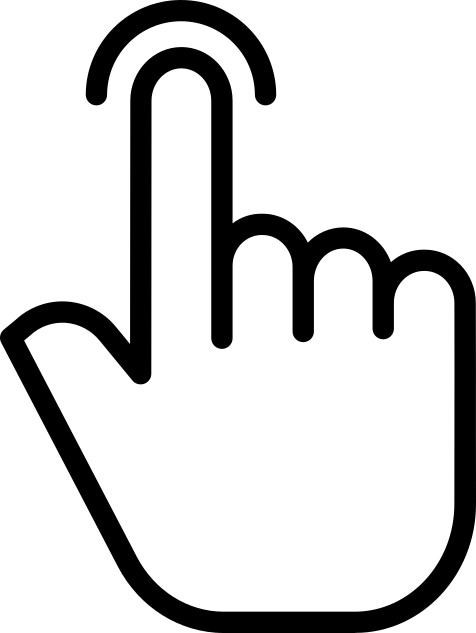
\includegraphics[width=0.05\textwidth]{img/dedo.png}} ;
     \node[invisible, below=of d, yshift=0.6cm] (inv_d) {} ;
     \node[factor, above=of d, xshift=-0.4cm] (fd0) {};
     \node[invisible, above=of fd0, xshift=-0.4cm, yshift=0.2cm] (inv_fd0) {};
    \node[factor, above=of d, xshift=0.4cm] (fd1) {};
     \node[invisible, above=of fd1, xshift=0.4cm, yshift=0.2cm] (inv_fd1) {};

     \node[latent, line width=0cm, yshift=4.8cm] (a) {
\includegraphics[width=0.06\textwidth]{img/prendido-apagado.png}};

    \vgate {fd} {(fd0)(inv_fd0)} {$0$} {(fd1)(inv_fd1)} {$1$} {a};

    \node[const, left=of fd] (nfd0) {$P(s_t|r_t)$};
    \node[const, right=of fd] (nfd1) {$P(s_t|r_t,c_t)$};

    \node[latent, above=of fd, xshift=-2.5cm, yshift=-0.2cm] (r) {
\includegraphics[width=0.06\textwidth]{img/regalo.png}} ;
    \node[factor, above=of r] (fr) {};
    \node[const, left=of fr] (nr) {\text{\Large $P(r_t)$}};

    \node[latent, fill=black!30, above=of fd, xshift=2.5cm, yshift=-0.2cm] (c) {
\includegraphics[width=0.06\textwidth]{img/cerradura.png}} ;
    \node[factor, above=of c] (fc) {};
    \node[const, right=of fc] (nc) {\text{\Large $P(c_t)$}};

    \node[latent, line width=0cm, yshift=4.8cm] (a) {
\includegraphics[width=0.06\textwidth]{img/prendido-apagado.png}};
    \node[factor, above=of a] (fa) {};

    \node[const, right=of fa] (na) {\text{\Large $P(a_t|p)$}};


    \node[latent, above=of fa, yshift=-0.3cm] (m) {
\includegraphics[width=0.06\textwidth]{img/cerebro.jpg}};
    \node[factor, above=of m] (fm) {};
    \node[const, right=of fm] (nm) {\text{\Large $P(p)$}};


    \edge[-] {r,c} {fd1};

    \edge[-] {r} {fd0};
    \edge {fd1} {d};

    \edge {fd0} {d};
    \edge {fc} {c};
    \edge {fr} {r};
    \edge {fm} {m};
    \edge {m} {a};

    \plate {B} {(inv_d)(a)(r)(c)(fa)(na)(nc)(nr)} {$t \in \{0, \dots, T-1\} $};
}
}
\caption{Red bayesiana causal, con intervenciones.}
\label{fig_ModeloCausalMemoria}
\end{figure}
%
\lipsum[2]

\begin{equation*}
P(\text{Modelo}|\text{Datos}) = \frac{P(\text{Datos}|\text{Modelo})P(\text{Modelo})}{P(\text{Datos})}
\end{equation*}


\lipsum[2]

\section{Resultados}

Al calcular el posterior de los modelos a medida que vamos incorporando nuevos datos observamos que,
%
\begin{figure}[H]
\centering
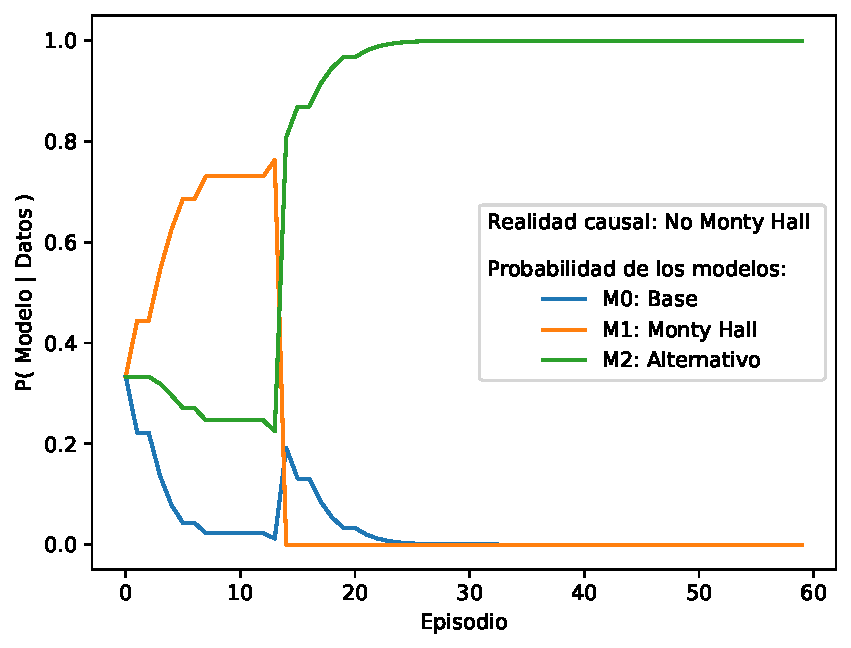
\includegraphics[width=0.5\textwidth]{img/posterior2.pdf}
\caption{Posterior de los modelos causales alternativos}
\end{figure}
%


\lipsum[2]


\lipsum[2]

\section{Conclusiones}


\lipsum[2]


\lipsum[2]

{\footnotesize
\bibliographystyle{plos2015.bst}
\bibliography{biblio}
}



\end{document}
